%iffalse
\let\negmedspace\undefined
\let\negthickspace\undefined
\documentclass[journal,12pt,onecolumn]{IEEEtran}
\usepackage[version=4]{mhchem}
\usepackage{chemformula} % for \ch if needed
\usepackage{chemfig}
\usepackage{chemmacros}
\chemsetup{modules = reactions} % Enables reaction arrows
\usepackage{graphicx}
\graphicspath{ {./images/} }

\usepackage{fancyhdr}
\usepackage{geometry}
\usepackage{lastpage}
\usepackage{cite}
\usepackage{amsmath,amssymb,amsfonts,amsthm}
\usepackage{enumitem,multicol}
\usepackage{algorithmic}
\usepackage{graphicx}
\usepackage{textcomp}
\usepackage{xcolor}
\usepackage{txfonts}
\usepackage{listings}
\usepackage{enumitem}
\usepackage{mathtools}
\usepackage{gensymb}
\usepackage{comment}
\usepackage[breaklinks=true]{hyperref}
\usepackage{tkz-euclide} 
\usepackage{listings}
\usepackage{gvv}                                        
%\def\inputGnumericTable{}                                 
\usepackage[latin1]{inputenc}                                
\usepackage{color}                                            
\usepackage{array}                                            
\usepackage{longtable}                                       
\usepackage{calc}                                             
\usepackage{multirow}                                         
\usepackage{hhline}                                           
\usepackage{ifthen}                                           
\usepackage{lscape}
\usepackage{tabularx}
\usepackage{array}
\usepackage{float}


\newtheorem{theorem}{Theorem}[section]
\newtheorem{problem}{Problem}
\newtheorem{proposition}{Proposition}[section]
\newtheorem{lemma}{Lemma}[section]
\newtheorem{corollary}[theorem]{Corollary}
\newtheorem{example}{Example}[section]
\newtheorem{definition}[problem]{Definition}
\newcommand{\BEQA}{\begin{eqnarray}}
\newcommand{\EEQA}{\end{eqnarray}}
\newcommand{\define}{\stackrel{\triangle}{=}}
\theoremstyle{remark}

\geometry{margin=1 in}

\pagestyle{fancy}
\fancyhead[L]{2019}
\fancyhead[C]{}
\fancyhead[R]{CY}
\fancyfoot[L]{CY}
\fancyfoot[C]{}
\fancyfoot[R]{\thepage/\pageref{LastPage}}

\setlength{\headheight}{14pt}
\setlength{\headsep}{5pt}
\setlength{\footskip}{20pt}


% Line thickness
\renewcommand{\headrulewidth}{0.4pt}
\renewcommand{\footrulewidth}{0.4pt}



% Marks the beginning of the document
\begin{document}



\title{
ASSIGNMENT 4: GATE 2019 \\
CY: CHEMISTRY}
\author{AI25BTECH11021 - Abhiram Reddy N}
\maketitle


\begin{enumerate} 





%----------------- Q1 ------------------
\item John Thomas, an \underline{\hspace{2cm}} writer, passed away in 2018.  \hfill{\brak{\textbf{GATE CY 2019}}}

\begin{multicols}{4}
\begin{enumerate}
    \item imminent
    \item prominent
    \item eminent
    \item dominant
\end{enumerate}
\end{multicols}

%----------------- Q2 ------------------
\item \underline{\hspace{1.5cm}} I permitted him to leave, I wouldn't have had any problem with him being absent, \underline{\hspace{1.5cm}} I?  \hfill{\brak{\textbf{GATE CY 2019}}}
\begin{multicols}{4}
\begin{enumerate}
    \item Had, wouldn't
    \item Have, would
    \item Had, would
    \item Have, wouldn't
\end{enumerate}
\end{multicols}

%----------------- Q3 ------------------
\item A worker noticed that the hour hand on the factory clock had moved by 225 degrees during her stay at the factory. For how long did she stay in the factory?  \hfill{\brak{\textbf{GATE CY 2019}}}
\begin{multicols}{4}
\begin{enumerate}
    \item 3.75 hours
    \item 4 hours and 15 mins
    \item 8.5 hours
    \item 7.5 hours
\end{enumerate}
\end{multicols}

%----------------- Q4 ------------------
\item The sum and product of two integers are 26 and 165 respectively. The difference between these two integers is \underline{\hspace{1.5cm}}.  \hfill{\brak{\textbf{GATE CY 2019}}}
\begin{multicols}{4}
\begin{enumerate}
    \item 2
    \item 3
    \item 4
    \item 6
\end{enumerate}
\end{multicols}

%----------------- Q5 ------------------
\item The minister avoided any mention of the issue of women's reservation in the private sector. He was accused of \underline{\hspace{2cm}} the issue.  \hfill{\brak{\textbf{GATE CY 2019}}}
\begin{multicols}{4}
\begin{enumerate}
    \item collaring
    \item skirting
    \item tying
    \item belting
\end{enumerate}
\end{multicols}

%----------------- Q6 ------------------
\item Under a certain legal system, prisoners are allowed to make one statement. If their statement turns out to be true then they are hanged. If the statement turns out to be false then they are shot. One prisoner made a statement and the judge had no option but to set him free. Which one of the following could be that statement?  \hfill{\brak{\textbf{GATE CY 2019}}}
\begin{multicols}{4}
\begin{enumerate}
    \item I did not commit the crime
    \item I committed the crime
    \item I will be shot
    \item You committed the crime
\end{enumerate}
\end{multicols}





%----------------- Q7 ------------------
\item A person divided an amount of Rs. 100,000 into two parts and invested in two different schemes. In one he got 10\% profit and in the other he got 12\%. If the profit percentages are interchanged with these investments he would have got Rs.120 less. Find the ratio between his investments in the two schemes.  \hfill{\brak{\textbf{GATE CY 2019}}}
\begin{multicols}{4}
\begin{enumerate}
    \item 9 : 16
    \item 11 : 14
    \item 37 : 63
    \item 47 : 53
\end{enumerate}
\end{multicols}

%----------------- Q8 ------------------
\item Congo was named by Europeans. Congo's dictator Mobuto later changed the name of the country and the river to Zaire with the objective of Africanising names of persons and spaces. However, the name Zaire was a Portuguese alteration of \textit{Nzadi o Nzere}, a local African term meaning 'River that swallows Rivers'. Zaire was the Portuguese name for the Congo river in the 16th and 17th centuries.\\
Which one of the following statements can be inferred from the paragraph above?  \hfill{\brak{\textbf{GATE CY 2019}}}

\begin{enumerate}
    \item Mobuto was not entirely successful in Africanising the name of his country
    \item The term \textit{Nzadi o Nzere} was of Portuguese origin
    \item Mobuto's desire to Africanise names was prevented by the Portuguese
    \item As a dictator Mobuto ordered the Portuguese to alter the name of the river to Zaire
\end{enumerate}



\vspace{2cm}


%----------------- Q9 ------------------
\item A firm hires employees at five different skill levels P, Q, R, S, T. The shares of employment at these skill levels of total employment in 2010 is given in the pie chart as shown. There were a total of 600 employees in 2010 and the total employment increased by 15\% from 2010 to 2016. The total employment at skill levels P, Q and R remained unchanged during this period. If the employment at skill level S increased by 40\% from 2010 to 2016, how many employees were there at skill level T in 2016? \hfill{\brak{\textbf{GATE CY 2019}}}

\begin{figure}[h!]
    \centering
    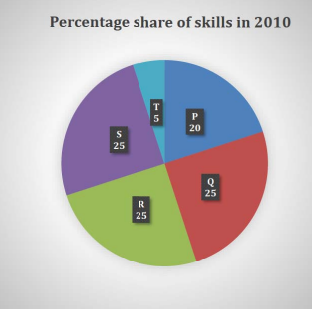
\includegraphics[width=0.5\textwidth]{figs/image1.png}
    \caption{Percentage share of skills in 2010.}
    \label{fig:q9piechart}
\end{figure}

\begin{multicols}{4}
\begin{enumerate}
    \item 30
    \item 35
    \item 60
    \item 72
\end{enumerate}
\end{multicols}
\newpage
%----------------- Q10 ------------------
\item M and N had four children P, Q, R and S. Of them, only P and R were married. They had children X and Y respectively. If Y is a legitimate child of W, which one of the following statements is necessarily FALSE? \hfill{\brak{\textbf{GATE CY 2019}}}
\begin{multicols}{4}
\begin{enumerate}
    \item M is the grandmother of Y
    \item R is the father of Y
    \item W is the wife of R
    \item W is the wife of P
\end{enumerate}
\end{multicols}

\end{enumerate}

\vspace{2cm}

\begin{center}
   \textbf{END OF THE QUESTION PAPER}
\end{center}


\begin{enumerate}
\newpage


%----------------- Q1 ------------------
\item The \textbf{INCORRECT} statement about the solid-state structure of CsCl and CaF$_2$ is: \hfill{\brak{\textbf{GATE CY 2019}}}

\begin{enumerate}
    \item Cations in both solids exhibit coordination number 8.
    \item CsCl has \textit{bcc} type structure and CaF$_2$ has cubic close pack structure.
    \item Radius ratio for Cs/Cl and Ca/F is 0.93 and 0.73, respectively.
    \item Both exhibit close pack structure.
\end{enumerate}


%----------------- Q2 ------------------
\item The \textbf{INCORRECT} statement about the interhalogen compound ICl$_3$ is: \hfill{\brak{\textbf{GATE CY 2019}}}

\begin{enumerate}
    \item It exists as a dimer.
    \item Geometry around the iodine is tetrahedral in solid-state.
    \item It decomposes as ICl and Cl$_2$ in gas-phase.
    \item Liquid ICl$_3$ conducts electricity.
\end{enumerate}


%----------------- Q3 ------------------
\item Among the following carbon allotropes, the one with discrete molecular structure is \hfill{\brak{\textbf{GATE CY 2019}}}

\begin{enumerate}
    \item Diamond
    \item $\alpha$-Graphite
    \item $\beta$-Graphite
    \item Fullerene
\end{enumerate}


%----------------- Q4 ------------------
\item The \textbf{INCORRECT} statement about the silicones is: \hfill{\brak{\textbf{GATE CY 2019}}}

\begin{enumerate}
    \item They are thermally unstable because of the Si--C bond.
    \item They are insoluble in water.
    \item They are organosilicon polymers.
    \item They have stable silica-like skeleton (-Si-O-Si-O-Si-).
\end{enumerate}


%----------------- Q5 ------------------
\item The $\Delta_0$ value of [Ni(H$_2$O)$_6$]$^{2+}$ is 8500 cm$^{-1}$. The $\Delta_0$ values for [NiCl$_6$]$^{4-}$ and [Ni(NH$_3$)$_6$]$^{2+}$ compared to [Ni(H$_2$O)$_6$]$^{2+}$ are \hfill{\brak{\textbf{GATE CY 2019}}}
\begin{multicols}{2}
\begin{enumerate}
    \item higher and lower, respectively.
    \item lower and higher, respectively.
    \item higher in both complex ions.
    \item lower in both complex ions.
\end{enumerate}
\end{multicols}






%----------------- Q6 ------------------
\item In Freundlich isotherm, a linear relationship is obtained in the plot of \\
$(\theta = \text{surface coverage and } p = \text{partial pressure of the gas})$ \hfill{\brak{\textbf{GATE CY 2019}}}
\begin{multicols}{4}
\begin{enumerate}
    \item $\theta$ vs $p$
    \item $\ln(\theta)$ vs $\ln(p)$
    \item $\ln(\theta)$ vs $p$
    \item $\theta$ vs $\ln(p)$
\end{enumerate}
\end{multicols}

%----------------- Q7 ------------------
\item Micelle formation is accompanied by the \hfill{\brak{\textbf{GATE CY 2019}}}

\begin{enumerate}
    \item decrease in overall entropy due to ordering.
    \item increase in overall entropy mostly due to increase in solvent entropy.
    \item increase in overall entropy mostly due to increase in solute entropy.
    \item increase in overall entropy and decrease in enthalpy.
\end{enumerate}

\newpage
%----------------- Q8 ------------------
\item Consider the following phase diagram of CO$_2$ (not to scale). At equilibrium, the \textbf{INCORRECT} statement is: \hfill{\brak{\textbf{GATE CY 2019}}}

\begin{figure}[h!]
    \centering
    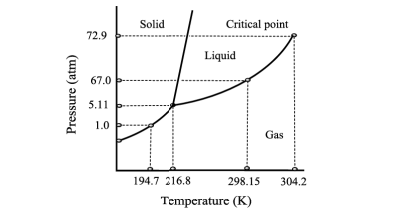
\includegraphics[width=0.5\textwidth]{figs/image2.png}
    \caption{Phase diagram of CO$_2$.}
    \label{fig:co2phasediagram}
\end{figure}


\begin{enumerate}
    \item At 200 K, on increasing the pressure from 1 to 50 atm, CO$_2$ gas condenses to liquid.
    \item It is not possible to obtain liquid CO$_2$ from gaseous CO$_2$ below 5.11 atm.
    \item Both liquid and gas phase of CO$_2$ coexist at 298.15 K and 67 atm.
    \item With increasing pressure, the melting point of solid CO$_2$ increases.
\end{enumerate}






%----------------- Q9 ------------------
\item The major product formed in the following reaction is \hfill{\brak{\textbf{GATE CY 2019}}}

\begin{figure}[h!]
    \centering
    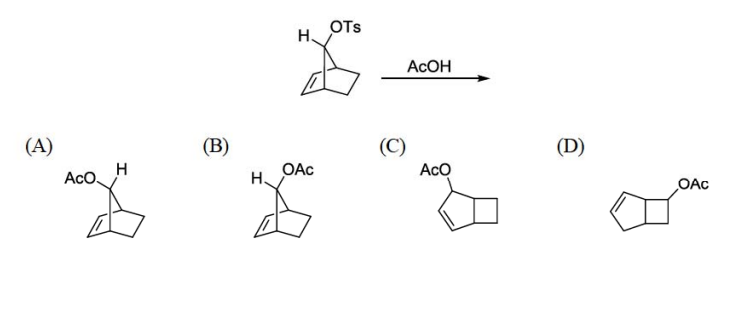
\includegraphics[width=0.8\textwidth]{figs/image3.png}
    \caption{Reaction for Q9}
    \label{fig:q9reaction}
\end{figure}



%----------------- Q10 ------------------
\item The Woodward-Hoffmann condition to bring out the following transformation is \hfill{\brak{\textbf{GATE CY 2019}}}


\begin{figure}[h!]
    \centering
    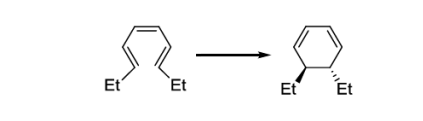
\includegraphics[width=0.7\textwidth]{figs/image4.png}
    \caption{Reaction for Q10}
    \label{fig:q10reaction}
\end{figure}



\begin{multicols}{2}
\begin{enumerate}
    \item $\Delta$, conrotatory
    \item $\Delta$, disrotatory
    \item hv, disrotatory
    \item hv, conrotatory
\end{enumerate}
\end{multicols}

%----------------- Q11 ------------------
\item The major product formed in the following reaction is \hfill{\brak{\textbf{GATE CY 2019}}}

\begin{figure}[h!]
    \centering
    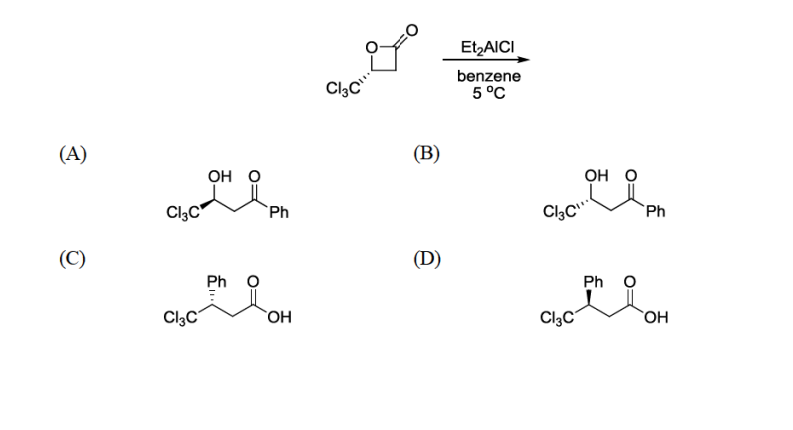
\includegraphics[width=0.9\textwidth]{figs/image5.png}
    \caption{Reaction for Q11}
    \label{fig:q11reaction}
\end{figure}

\newpage

%----------------- Q12 ------------------
\item In the following reaction, the stereochemistry of the major product is predicted by the \hfill{\brak{\textbf{GATE CY 2019}}}

\begin{figure}[h!]
    \centering
    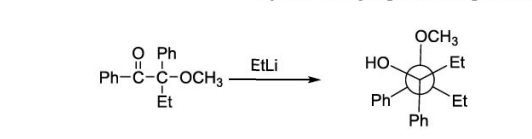
\includegraphics[width=0.9\textwidth]{figs/image6.png}
    \caption{Reaction for Q12}
    \label{fig:q12reaction}
\end{figure}

\begin{multicols}{2}
\begin{enumerate}
    \item Cram's model
    \item Cram's chelation model
    \item Felkin model
    \item Felkin-Ahn model
\end{enumerate}
\end{multicols}

%----------------- Q13 ------------------
\item The product(s) formed in the following reaction is (are) \hfill{\brak{\textbf{GATE CY 2019}}}

\begin{figure}[h!]
    \centering
    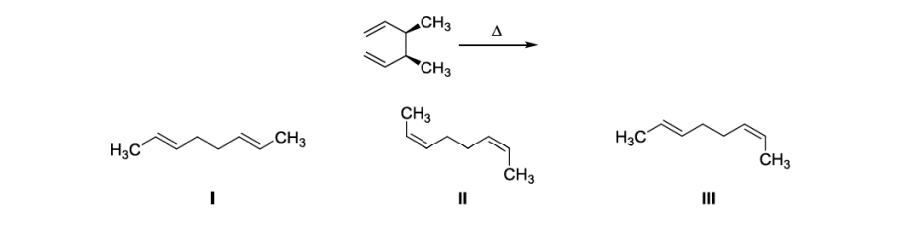
\includegraphics[width=0.8\textwidth]{figs/image7.png}
    \caption{Reaction for Q13}
    \label{fig:q13reaction}
\end{figure}

\begin{multicols}{2}
\begin{enumerate}
    \item I only
    \item II only
    \item III only
    \item mixture of I and II
\end{enumerate}
\end{multicols}
\newpage
%----------------- Q14 ------------------
\item Among the following compounds, the number of compounds that DO NOT exhibit optical activity at room temperature is \hfill{\brak{\textbf{GATE CY 2019}}}

\begin{figure}[h!]
    \centering
    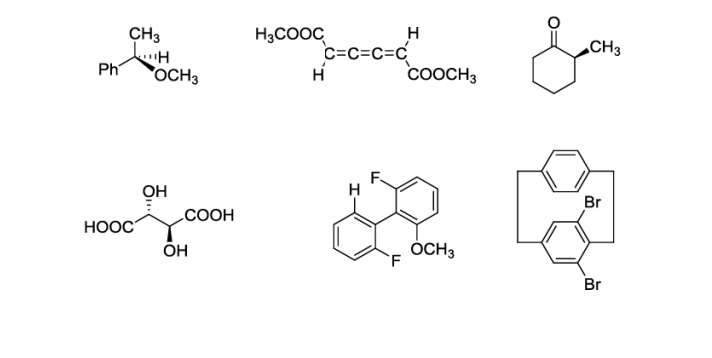
\includegraphics[width=0.8\textwidth]{figs/image8.png}
    \caption{Compounds for Q14}
    \label{fig:q14compounds}
\end{figure}





%----------------- Q15 ------------------
\item The number of following diene(s) that undergo Diels-Alder reaction with methyl acrylate is \hfill{\brak{\textbf{GATE CY 2019}}}

\begin{figure}[h!]
    \centering
    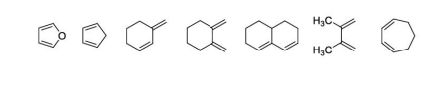
\includegraphics[width=0.8\textwidth]{figs/image9.png}
    \caption{Dienes for Q15}
    \label{fig:q15dienes}
\end{figure}

%----------------- Q16 ------------------
\item The number of \(^1H\) NMR signals observed for the following compound is \hfill{\brak{\textbf{GATE CY 2019}}}

\begin{figure}[h!]
    \centering
    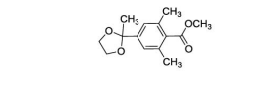
\includegraphics[width=0.6\textwidth]{figs/image10.png}
    \caption{Compound for Q16}
    \label{fig:q16compound}
\end{figure}

\newpage
%----------------- Q17 ------------------
\item The number of CO stretching bands in IR spectrum of trigonal bipyramidal \textit{cis}-M(CO)$_3$L$_2$ is \hfill{\brak{\textbf{GATE CY 2019}}}

(M = metal and L = monodentate ligand)

%----------------- Q18 ------------------
\item On heating a sample of 25 mg hydrated compound (molecular weight = 250 g/mol) in thermogravimetric analysis, 16 mg of dehydrated compound remains. The number of water molecules lost per molecule of hydrated compound is \hfill{\brak{\textbf{GATE CY 2019}}}

(Molecular weight of water = 18 g/mol)

%----------------- Q19 ------------------
\item The total number of $\alpha$ and $\beta$ particles emitted in the following radioactive decay is \hfill{\brak{\textbf{GATE CY 2019}}}

\begin{figure}[h!]
    \centering
    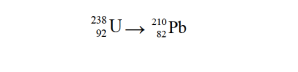
\includegraphics[width=0.6\textwidth]{figs/image11.png}
    \caption{Radioactive decay for Q19}
    \label{fig:q19decay}
\end{figure}






%----------------- Q20 ------------------
\item An ideal gas occupies an unknown volume \(V\) liters (L) at a pressure of 12 atm. The gas is expanded isothermally against a constant external pressure of 2 atm so that its final volume becomes 31 L. The work involved for this expansion process is cal. (Round off to two decimal places) \hfill{\brak{\textbf{GATE CY 2019}}}

(Gas constant \(R = 0.082 \text{ L atm mol}^{-1} \text{K}^{-1} 2 \text{ cal mol}^{-1} \text{K}^{-1}\))

%----------------- Q21 ------------------
\item The entropy change for the melting of \(x\) moles of ice (heat of fusion is 80 cal g\(^{-1}\)) at 273 K and 1 atm pressure is 28.80 cal K\(^{-1}\). The value of \(x\) is . (Round off to two decimal places)

(Molecular weight of water = 18 g/mol) \hfill{\brak{\textbf{GATE CY 2019}}}

%----------------- Q22 ------------------
\item Consider a two-state system at thermal equilibrium having energies 0 and 2\(kT\) for which the degeneracies are 1 and 2, respectively. The value of the partition function at the same absolute temperature T is . (Round off to two decimal places)

(\(k\) is the Boltzmann constant) \hfill{\brak{\textbf{GATE CY 2019}}}

%----------------- Q23 ------------------
\item Consider a system of three identical and cistriglyceride non-interacting particles and three available nondegenerate single particle energy levels having energies 0, 0, and 2\(\epsilon\). The system is in contact with a heat bath of temperature \(T\). A total energy of 2\(\epsilon\) is shared by these three particles. The number of ways five particles can be distributed is . \hfill{\brak{\textbf{GATE CY 2019}}}

%----------------- Q24 ------------------
\item In a 400 MHz \(^1H\) NMR spectrometer, a proton resonates at 1560 Hz higher than that of tetramethylsilane. The chemical shift value of this proton is  ppm. (Round off to one decimal place)

(Chemical shift of tetramethylsilane is fixed at zero ppm) \hfill{\brak{\textbf{GATE CY 2019}}}

%----------------- Q25 ------------------
\item Gas phase bond length and dipole moment of a compound (MX) is 3 A and 10.8 D, respectively. The ionic character in gas phase MX is  %. (Round off to one decimal place)

(1 D = 3.336 \(\times 10^{-30}\) C m) \hfill{\brak{\textbf{GATE CY 2019}}}





%----------------- Q26 ------------------
\item The experimentally observed magnetic moment values, which match well with the spin-only values for the pair of argon ions is \hfill{\brak{\textbf{GATE CY 2019}}}
\begin{multicols}{2}
\begin{enumerate}
\item  Cr(III) and Cr(II)
\item  Cr(III) and Cr(III)
\item  Cr(III) and Dy(III)
\item  La(III) and Tb(III)
\end{enumerate}
\end{multicols}

%----------------- Q27 ------------------
\item Among the following compounds, a normal spinel is \hfill{\brak{\textbf{GATE CY 2019}}}
\begin{multicols}{4}
\begin{enumerate}
\item  MgFe\(_2\)O\(_4\)
\item  ZnFe\(_2\)O\(_4\)
\item  CoFe\(_2\)O\(_4\)
\item  Co\(_3\)O\(_4\)
\end{enumerate}
\end{multicols}

%----------------- Q28 ------------------
\item Following are the examples of silicate minerals \hfill{\brak{\textbf{GATE CY 2019}}}

\begin{multicols}{3}
I. Zircon, ZrSiO\(_4\) \\
II. Beryl, Be\(_3\)Al\(_2\)Si\(_6\)O\(_{18}\) \\
III. Pyroxferdite, Al\(_2\)O(OH)(SiO\(_4\)) \\
\end{multicols}

The correct structural description of the minerals is

\begin{enumerate}
\item  I - Ortho silicate, II - Cycle silicate and III - Sheet silicate
\item  I - Ortho silicate, II - Sheet silicate and III - Cycle silicate
\item  I - Cycle silicate, II - Sheet silicate and III - Ortho silicate
\item  I - Sheet silicate, II - Ortho silicate and III - Cycle silicate
\end{enumerate}


%----------------- Q29 ------------------
\item In the EPR spectrum of a methyl radical, the number of lines and their relative intensities respectively, are \hfill{\brak{\textbf{GATE CY 2019}}}

\begin{enumerate}
\item  1 and 1:2:1
\item  3 and 1:1:1
\item  4 and 1:2:2:1
\item  4 and 1:3:3:1
\end{enumerate}


%----------------- Q30 ------------------
\item The product obtained in the reaction of M(s)CO\(_3\) with Br\(_2\) is \hfill{\brak{\textbf{GATE CY 2019}}}

\begin{enumerate}
\item  M(s)CO\(_3\)Br
\item  M(s)(CO\(_3\))Br\(_2\)
\item  M(s)CO(Br)\(_2\)
\item  M(s)(CO\(_3\))Br
\end{enumerate}




%----------------- Q31 ------------------
\item The correct molecular representation of W(Cp)$_2$(CO)$_2$ is \hfill{\brak{\textbf{GATE CY 2019}}}

\begin{enumerate}
\item [(A)] [W($\eta^1$-Cp)($\eta^3$-Cp)(CO)$_2$]
\item [(B)] [W($\eta^1$-Cp)($\eta^5$-Cp)(CO)$_2$]
\item [(C)] [W($\eta^3$-Cp)($\eta^5$-Cp)(CO)$_2$]
\item [(D)] [W($\eta^5$-Cp)$_2$(CO)$_2$]
\end{enumerate}




%----------------- Q32 ------------------
\item Match the metalloproteins with their respective functions. \hfill{\brak{\textbf{GATE CY 2019}}}

\begin{center}
\begin{tabular}{|c|c|c|c|}
\hline
P & Ferritin & I & Electron transfer \\
Q & Rubredoxin & II & Acid-base catalysis \\
R & Cobalamin & III & Metal storage \\
S & Carbonic anhydrase & IV & Methyl transfer \\
\hline
\end{tabular}
\end{center}

\begin{multicols}{2}
\begin{enumerate}
\item [(A)] P - III; Q - II; R - I; S - IV
\item [(B)] P - III; Q - I; R - IV; S - II
\item [(C)] P - IV; Q - I; R - III; S - II
\item [(D)] P - IV; Q - II; R - I; S - III
\end{enumerate}
\end{multicols}

\newpage


%----------------- Q33 ------------------
\item Suppose the wave function of a one dimensional system is 
\[
\psi = \sin(kx) \exp(3ikx).
\]
In an experiment measuring the momentum of the system, one of the expected outcomes is \hfill{\brak{\textbf{GATE CY 2019}}}
\begin{multicols}{4}
\begin{enumerate}
\item 0
\item $\hbar k$
\item $2 \hbar k$
\item $3 \hbar k$
\end{enumerate}
\end{multicols}





%----------------- Q34 ------------------
\item The major product formed in the following reaction is \hfill{\brak{\textbf{GATE CY 2019}}}

\begin{figure}[H]
    \centering
    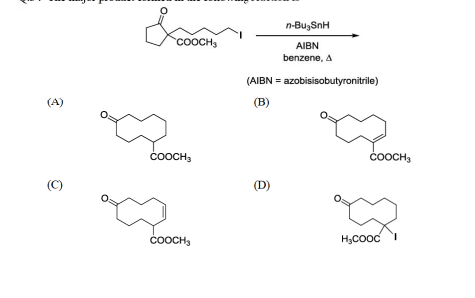
\includegraphics[width=0.8\linewidth]{figs/image12.png}
    \caption{Reaction for Q34}
    \label{fig:q34}
\end{figure}

%----------------- Q35 ------------------
\item The major product formed in the following reaction is \hfill{\brak{\textbf{GATE CY 2019}}}

\begin{figure}[H]
    \centering
    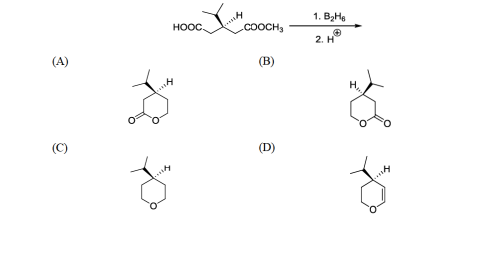
\includegraphics[width=0.7\linewidth]{figs/image13.png}
    \caption{Reaction for Q35}
    \label{fig:q35}
\end{figure}








%----------------- Q36 ------------------
\item The major product formed in the following reaction is \hfill{\brak{\textbf{GATE CY 2019}}}

\begin{figure}[H]
    \centering
    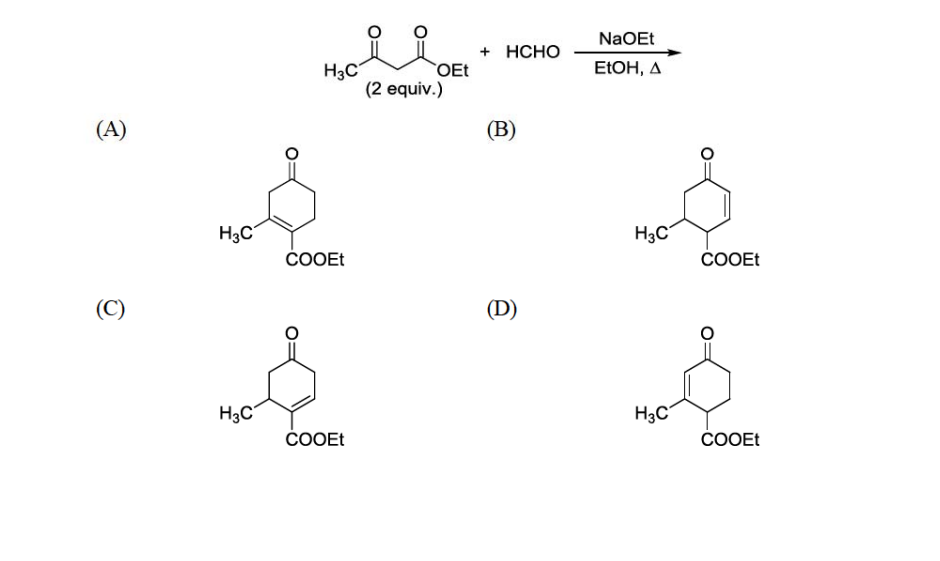
\includegraphics[width=0.8\linewidth]{figs/image14.png}
    \caption{Reaction for Q36}
    \label{fig:q36}
\end{figure}


%----------------- Q37 ------------------
\item The major product formed in the following reaction is \hfill{\brak{\textbf{GATE CY 2019}}}

\begin{figure}[H]
    \centering
    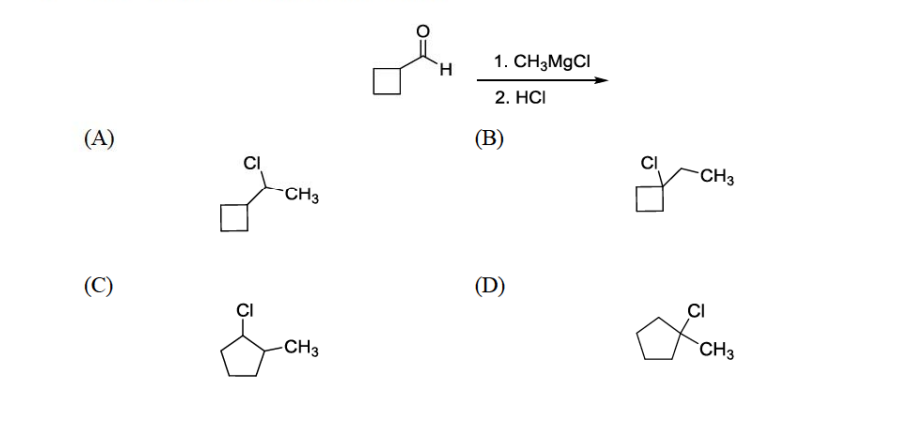
\includegraphics[width=0.8\linewidth]{figs/image15.png}
    \caption{Reaction for Q37}
    \label{fig:q37}
\end{figure}



%----------------- Q38 ------------------
\item In the following reaction sequence, the products \textit{P} and \textit{Q} are \hfill{\brak{\textbf{GATE CY 2019}}}

\begin{figure}[H]
    \centering
    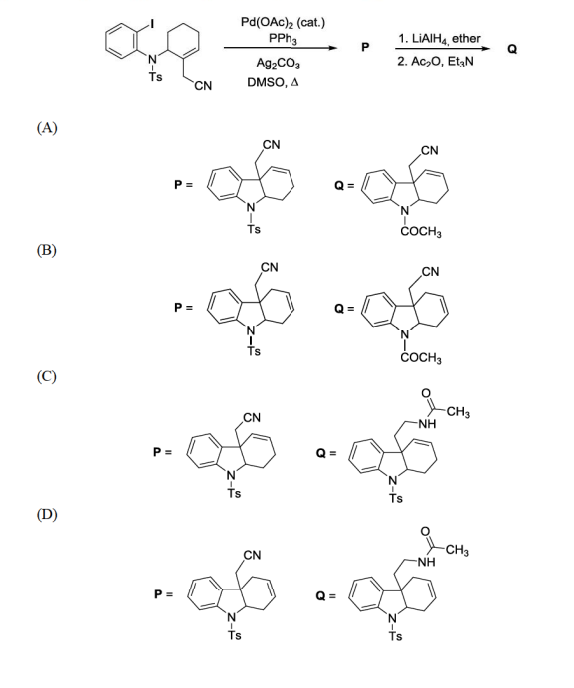
\includegraphics[width=0.8\linewidth]{figs/image16.png}
    \caption{Reaction sequence for Q38}
    \label{fig:q38}
\end{figure}



%----------------- Q39 ------------------
\item The major product formed in the following reaction is \hfill{\brak{\textbf{GATE CY 2019}}}

\begin{figure}[H]
    \centering
    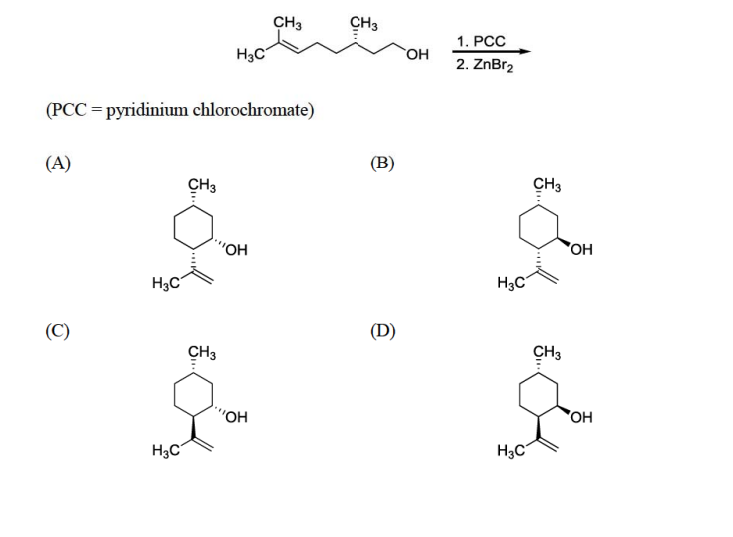
\includegraphics[width=0.8\linewidth]{figs/image17.png}
    \caption{Reaction for Q39}
    \label{fig:q39}
\end{figure}



%----------------- Q40 ------------------
\item In the following reactions, the major products \textit{P} and \textit{Q} are \hfill{\brak{\textbf{GATE CY 2019}}}

\begin{figure}[H]
    \centering
    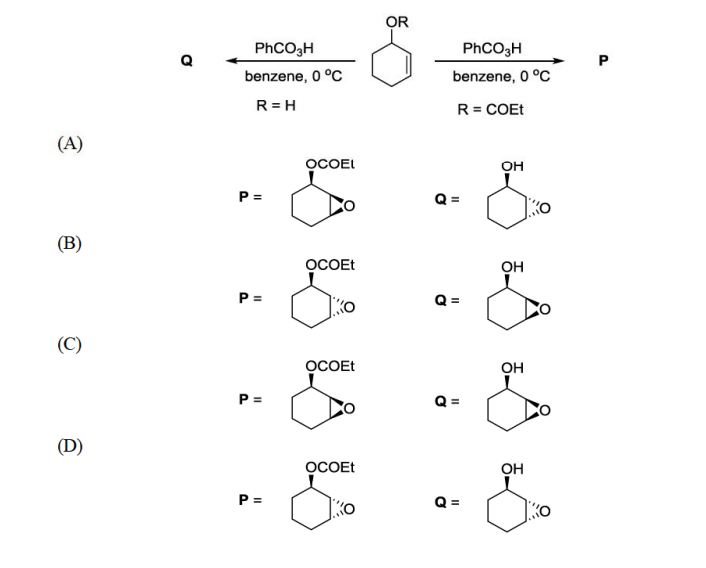
\includegraphics[width=0.8\linewidth]{figs/image18.png}
    \caption{Reactions for Q40}
    \label{fig:q40}
\end{figure}

%----------------- Q41 ------------------
\item In the following reaction sequence, the products \textit{P} and \textit{Q} are \hfill{\brak{\textbf{GATE CY 2019}}}

\begin{figure}[H]
    \centering
    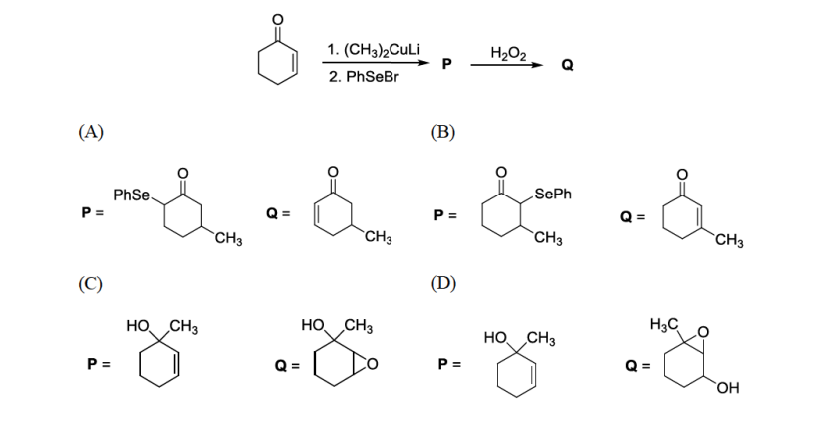
\includegraphics[width=0.9\linewidth]{figs/image19.png}
    \caption{Reaction sequence for Q41}
    \label{fig:q41}
\end{figure}





%----------------- Q42 ------------------
\item The major product formed in the following reaction is \hfill{\brak{\textbf{GATE CY 2019}}}

\begin{figure}[H]
    \centering
    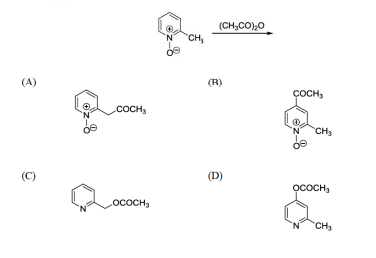
\includegraphics[width=0.8\linewidth]{figs/image20 .png}
    \caption{Reaction for Q42}
    \label{fig:q42}
\end{figure}


%----------------- Q43 ------------------
\item The rate of the following redox reaction is slowest when \textit{X} is \hfill{\brak{\textbf{GATE CY 2019}}}

\[
\text{[Co}^{\text{III}}\text{(NH}_3)_5\text{X]}^{3+/2+} + [\text{Cr}^{\text{II}}\text{(H}_2\text{O})_6]^{2+} \rightarrow [\text{Co}^{\text{II}}\text{(NH}_3)_5\text{(H}_2\text{O})]^{2+} + [\text{Cr}^{\text{III}}\text{(H}_2\text{O})_5\text{X}]^{3+/2+}
\]

\begin{multicols}{2}
\begin{enumerate}
\item \(\text{H}_2\text{O}\)
\item \(\text{NH}_3\)
\item \(\text{Cl}^-\)
\item \(\text{N}_3^-\)
\end{enumerate}
\end{multicols}

%----------------- Q44 ------------------
\item A complex is composed of one chromium ion, three bromides and six water molecules. Upon addition of excess AgNO\(_3\), 1.0 g aqueous solution of the complex gave 0.94 g of AgBr. The molecular formula of the complex is \hfill{\brak{\textbf{GATE CY 2019}}}

(Atomic weight: Cr = 52, Br = 80, Ag = 108, O = 16 and H = 1)

\begin{multicols}{2}
\begin{enumerate}
\item \(\mathrm{[Cr(H_2O)_6]Br_3}\)
\item \(\mathrm{[Cr(H_2O)_5Br]Br_2 \cdot H_2O}\)
\item \(\mathrm{[Cr(H_2O)_4Br_2]Br \cdot 2H_2O}\)
\item \(\mathrm{[Cr(H_2O)_3Br_3] \cdot 3H_2O}\)
\end{enumerate}
\end{multicols}





%----------------- Q45 ------------------
\item The number of possible optically active isomer(s) for the following complex is \rule{2cm}{0.15mm}. \hfill{\brak{\textbf{GATE CY 2019}}}

\begin{figure}[H]
    \centering
    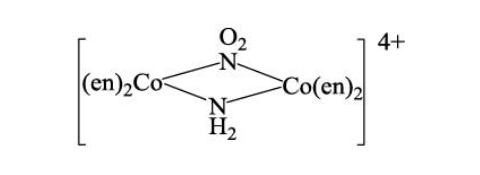
\includegraphics[width=0.5\linewidth]{figs/image21.png}
    \caption{Structure of the coordination complex in Q45}
    \label{fig:q45}
\end{figure}

\textbf{Note:} en = ethylenediamine

%----------------- Q46 ------------------
\item The specific rotation of optically pure (R)-2-bromobutane is -112.00. A given sample of 2-bromobutane exhibited a specific rotation of -82.88. The percentage of (S)-(+) enantiomer present in this sample is \rule{2cm}{0.15mm}. \hfill{\brak{\textbf{GATE CY 2019}}}

%----------------- Q47 ------------------
\item Consider the following two parallel irreversible first order reactions at temperature T, \hfill{\brak{\textbf{GATE CY 2019}}}

\begin{figure}[H]
    \centering
    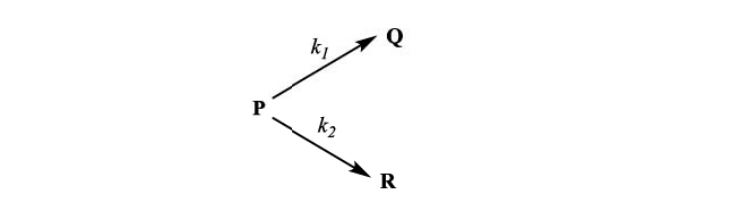
\includegraphics[width=0.35\linewidth]{figs/image22.png}
    \caption{Reaction scheme for Q47}
    \label{fig:q47}
\end{figure}

\noindent where \(k_1\) and \(k_2\) are the rate constants and their values are \(5 \times 10^{-2}~\text{min}^{-1}\) and \(15 \times 10^{-2}~\text{min}^{-1}\), respectively, at temperature T. If the initial concentration of the reactant \(P\) is \(4~\text{mol L}^{-1}\), then the concentration of product \(R\) after 10 min of reaction is \rule{2cm}{0.15mm} mol L\(^{-1}\). (Round off to two decimal places)

\textbf{(Assume only P is present at the beginning of the reaction.)}

%----------------- Q48 ------------------
\item Consider the following equilibrium \hfill{\brak{\textbf{GATE CY 2019}}}

\[
\text{SO}_2 (g) + \frac{1}{2} \text{O}_2 (g) \rightleftharpoons \text{SO}_3 (g)
\]

At 298 K, the standard molar Gibbs energies of formation, \(\Delta G_f^\circ\), of SO\(_2\) (g) and SO\(_3\) (g) are -300 and -371 kJ mol\(^{-1}\), respectively. The value of the equilibrium constant, \(K_p\), at this temperature is \rule{2cm}{0.15mm} \(\times 10^{10}\). (Round off to the nearest integer)

\textbf{(Gas constant R = 8.31 J mol\(^{-1}\) K\(^{-1}\))}




%----------------- Q49 ------------------
\item Consider the electrochemical cell
\[
\text{M(s)}|\text{M}^{2+}(s)|\text{M}|\text{M(s)}
\]
where `M' is a metal. At 298 K, the standard reduction potentials are 
\[
E^\circ_{\text{M}^{2+}(aq)/M(s)} = -0.12~V, \quad
E^\circ_{\text{M}^{2+}_{(s)}/M(s)} = -0.36~V
\]
and the temperature coefficient is
\[
\left(\frac{\partial E^\circ_{\text{cell}}}{\partial T}\right)_P = 1.5 \times 10^{-4} \, V\,K^{-1}.
\]
At this temperature the standard enthalpy change for the overall cell reaction, \(\Delta_r H^\circ\), is \rule{2cm}{0.15mm} kJ mol\(^{-1}\). (Round off to two decimal places)

(Faraday constant F = 96500 C mol\(^{-1}\))

%----------------- Q50 ------------------
\item The normal boiling point of a compound (X) is 350 K (heat of vaporization, \(\Delta_{vap}H_v = 30\) kJ mol\(^{-1}\)). The pressure required to boil 'X' at 300 K is \rule{2cm}{0.15mm} Torr. (Round off to two decimal places)

(Ignore the temperature variation of \(\Delta_{vap}H_v\); Gas constant R = 8.31 J mol\(^{-1}\) K\(^{-1}\) and 1 atm = 760 Torr)

%----------------- Q51 ------------------
\item For a bimolecular gas phase reaction \(P + Q \rightarrow R\), the pre-exponential factor is \(1 \times 10^{13}\) dm\(^3\) mol\(^{-1}\) s\(^{-1}\). The standard entropy of activation at 25 \(^{\circ}\)C is \rule{2cm}{0.15mm} J K\(^{-1}\) mol\(^{-1}\). (Round off to two decimal points)

(The standard concentration \(c^\circ = 1\) mol dm\(^{-3}\); Planck constant \(h = 6.62 \times 10^{-34}\) J s; Boltzmann constant \(k_B = 1.38 \times 10^{-23}\) J K\(^{-1}\); Gas constant \(R = 8.31\) J mol\(^{-1}\) K\(^{-1}\))

%----------------- Q52 ------------------
\item Character table of point group D\(_8\) is given below.

\begin{table}[H]
    \centering
    \setlength{\tabcolsep}{6pt}
    \renewcommand{\arraystretch}{1.3}
    \begin{tabular}{c|cccccccccc}
        D\(_8\) & E & 2C\(_8\) & 2C\(_4\) & 2C\(_8^3\) & C\(_2\) & 4C\(_2'\) & 4C\(_2''\) \\
        \hline
        A\(_1\) & \textbf{a} & 1 & 1 & 1 & 1 & 1 & 1 \\
        A\(_2\) & \textbf{b} & 1 & 1 & 1 & 1 & \textbf{h} & \textbf{i} \\
        B\(_1\) & \textbf{c} & -1 & 1 & -1 & 1 & 1 & j \\
        B\(_2\) & \textbf{d} & -1 & -1 & 1 & -1 & 1 & 0 \\
        E\(_1\) & \textbf{e} & \(\sqrt{2}\) & 0 & \(-\sqrt{2}\) & -2 & 0 & 0 \\
        E\(_2\) & \textbf{f} & 0 & -2 & 0 & \textbf{k} & 0 & 0 \\
        E\(_3\) & \textbf{g} & \(-\sqrt{2}\) & 0 & \(\sqrt{2}\) & -2 & 0 & 0 \\
    \end{tabular}
\end{table}

Value of \(\textbf{(a + b + c + d + e + f + g + h + i + j + k)}\) is equal to \rule{2cm}{0.15mm}.




%----------------- Q53 ------------------
\item If \(\langle \alpha | \hat{S}_x \hat{S}_y - \hat{S}_y \hat{S}_x | \alpha \rangle = i\hbar^2 a\), where \(\hat{S}_x\) and \(\hat{S}_y\) are spin angular momentum operators and \(|\alpha\rangle\) is spin up eigenfunction, then the value of '\(a\)' is \rule{2cm}{0.15mm}. (Round off to one decimal place)

%----------------- Q54 ------------------
\item A particle in one dimensional box of length \(2a\) with potential energy
\[
V = \begin{cases}
0 & |x| < a \\
\infty & |x| > a
\end{cases}
\]
is perturbed by the potential \(V' = cx\) eV, where \(c\) is a constant. The 1\textsuperscript{st} order correction to the 1\textsuperscript{st} excited state of the system is \rule{2cm}{0.15mm} \(\times c\) eV.

%----------------- Q55 ------------------
\item Consider a two dimensional harmonic oscillator with angular frequency \(\omega_x = 2\omega_y = 6.5 \times 10^{14}\) rad s\(^{-1}\). The wavelength of \(x\) polarized light required for the excitation of a particle from its ground state to the next allowed excited state is \rule{2cm}{0.15mm} \(\times 10^{-6}\) m. (Round off to one decimal place)

(Speed of light \(c = 3.0 \times 10^{8}\) m s\(^{-1}\))

\bigskip

\begin{center}
\textbf{END OF THE QUESTION PAPER}
\end{center}











  
\end{enumerate}

\end{document}